\chapter{Introducción y contexto}\label{chap:Intro}

Visión computacional es el conjunto de metodos y tecnicas por las cuales se intenta comprender y analizar las imagenes del mundo real mediante el uso de una computadora.
Representa un problema bastante difícil, en parte porque es un problema inverso en el cual intentamos recuperar algunas incógnitas de cómo llegar a una solución especifica, esto quiere decir que sabemos cual es la solución, por ejemplo reconocer un auto o segmentar una figura, pero no conocemos la totalidad del proceso por el cual hemos llegado a dicha solución (\cite{szeliski2010computer}). 

Según \cite{szeliski2010computer} las áreas más comunes de visión computacional son: 
\begin{itemize}
\item Procesamiento de imágenes.
\item Detección de características.
\item Segmentación.
\item Alineamiento en base a características.
\item Estimación del movimiento.
\item Fusión de imágenes.
\item Fotografía computacional.
\item Estéreo correspondencia.
\item Modelamiento de formas 3D.
\item \textit{Rendering} basado en imágenes.
\item Reconocimiento.
\end{itemize}

Donde el reconocimiento es la tarea de encontrar e identificar objetos en particular en una imagen o secuencia de vídeo. Mientras los seres humanos podemos reconocer varios objetos en una imagen sin esfuerzo. Replicar este proceso en una maquina con toda su versatilidad sigue siendo un gran desafío.
Entre las varias formas de reconocimiento existe el reconocimiento de rostros que se presenta de dos maneras, una es verificación y la otra es identificación (\cite{alice2003biometric}).

Mientras la verificación intenta contestar sí una imagen de un rostro pertenece una persona en particular, la identificación intenta contestar la pregunta ¿ a quién le pertenece la imagen del rostro? siendo un proceso más complejo que la verificación debido a que mientras uno es una comparación uno a uno entre la imagen a examinar y el rostro del sujeto a verificar, el otro es una comparación de uno a varios entre la imagen del rostro y el conjunto de rostros que se tengan para identificar teniendo en cuenta la posibilidad de que el rostro a identificar no pertenezca al conjunto de rostros con los que se realiza la comparación.

% \usepackage{multirow}
\begin{table}[h]
\centering
\caption{Aplicaciones típicas del reconocimiento de rostros según \cite{zhao2003face}}
\label{TaAplicaciones}
\centering
  \resizebox{\textwidth}{!}{ 
\begin{tabular}{|c|l|}
\hline
\textbf{Áreas}                                              & \multicolumn{1}{c|}{\textbf{Aplicaciones especificas}}                          \\ \hline
\multirow{2}{*}{\textbf{Entretenimiento}}                   & Vídeo juegos, realidad virtual, programas de entrenamiento                      \\ \cline{2-2} 
                                                            & Interacciones robot-humano, Interacciones humano-computadora                    \\ \hline
\multirow{3}{*}{\textbf{Tarjetas inteligentes}}             & Licencias de conducir, Programas de autorización                                \\ \cline{2-2} 
                                                            & Inmigración, Documento de identificación, Pasaportes, registro de votantes      \\ \cline{2-2} 
                                                            & Seguro contra fraude                                                            \\ \hline
\multirow{4}{*}{\textbf{Seguridad de la información}}       & TV de control parental, Ingreso a dispositivos personales, Ingreso a desktop    \\ \cline{2-2} 
                                                            & Aplicaciones de seguridad, Seguridad de base de datos, encriptación de archivos \\ \cline{2-2} 
                                                            & Seguridad de Intranet, Acceso a Internet, Registros médicos                    \\ \cline{2-2} 
                                                            & Seguridad de terminales de comercio                                             \\ \hline
\multirow{3}{*}{\textbf{Aplicación de la ley y vigilancia}} & \textbf{Vídeo vigilancia avanzada, control de CCTV}                             \\ \cline{2-2} 
                                                            & Control de Portales, Análisis Post evento                                       \\ \cline{2-2} 
                                                            & Robo de tiendas, Investigación y seguimiento de sospechosos                     \\ \hline
\end{tabular}
}
\end{table}

Según el \textit{survey} de \cite{zhao2003face}, entre las varias aplicaciones del reconocimiento de rostros, Cuadro \ref{TaAplicaciones}, se menciona su aplicación en video vigilancia y \ac{CCTV}. En estas aplicaciones usualmente el proceso de reconocimiento es llevado a cabo por seres humanos, esto implica que la calidad del trabajo no será la misma en todo momento, y aumenta la posibilidad de un error por factor humano. Se explica en mayor detalle este problema y la necesidad de automatizar este proceso en la Sección \ref{ssc:PlanteamientoProblema}.

El uso de cámaras para monitorear lugares de interés no es nuevo, de hecho se ha realizado durante décadas, este arreglo entre cámaras de seguridad y la infraestructura necesaria para su funcionamiento y visualización de las imágenes se conoce como \ac{CCTV}. 

Inicialmente su uso estaba reservado para complejos industriales debido al alto coste de los equipos que se necesitaba, en especial las cámaras. Pero hoy la situación es contraria, ahora se usa desde espacios públicos hasta edificios privados y hogares. Su difusión ha ido aumentando con el paso del tiempo por el menor costo del \textit{hardware} y una mayor preocupación por un control de seguridad. Esta mayor preocupación motiva la investigación de técnicas que permita identificar a las personas sin su cooperación.

Existen muchas iniciativas para el uso del reconocimiento de rostros en ambientes no controlados, esto quiere decir que no se tiene control sobre las condiciones de iluminación, angulo de visión, oclusiones e incluso la colaboración de los sujetos a reconocer entre otros factores.
 
En trabajos como el de \cite{gorodnichy2014survey} para el gobierno de Canadá, se puede ver la necesidad de contar con un sistema fiable de vídeo vigilancia en este caso para puestos fronterizos. En  \cite{tian2005robust} se presenta un método para el análisis de fondo de una escena de vídeo proporcionado por una cámara de vigilancia estática, y en \cite{nazare2014smart} se presenta una propuesta de \textit{framework} para la unión de varios procesos de visión computacional agrupándolos en módulos: reconocimiento de áreas de interés, seguimiento e identificación y extracción de conocimiento, todos ellos aplicados a vídeo vigilancia.

El uso visión computacional en vídeo vigilancia no solo se limita al ámbito académico, existen varias situaciones donde la necesidad de seguridad ha creado la infraestructura necesaria para que investigaciones como las citadas anteriormente tengan un uso practico. Un ejemplo es \cite{odobez2012unsupervised} que es la demostración del prototipo de un sistema de vídeo vigilancia para un metro. Todo este incremento también ha despertado un gran interés sobre el alcance de la vídeo vigilancia como en el caso de la cuidad de Londres, donde \cite{wood2006report} muestra la gran cantidad de cámaras instaladas en la cuidad y habla sobre los posible problemas concernientes a la privacidad en una sociedad donde la vigilancia en pro de la seguridad es una prioridad, un caso similar es el de la cuidad de Chicago expuesto en \cite{schwartz2012chicago}.

Se ha mencionado el contexto de esta tesis que es el reconocimiento de rostros en vídeo vigilancia en ambientes no controlados, que nace de la necesidad de un control de seguridad automatizado y también debido a la oportunidad generada por las existencia de una creciente infraestructura en cámaras de vigilancia junto al hecho que los trabajos de visión computacional son lo suficientemente maduros como para ponerse en practica.


\section{Planteamiento del problema}\label{ssc:PlanteamientoProblema}
El problema de reconocimiento de rostro en vídeo vigilancia aun no ha sido resuelto en visión computacional e inclusive resulta un problema para el ser humano como se explica en \cite{burton1999face} donde se prueba que las personas tienen problemas para reconocer sujeto con los que no son familiares en videos de baja resolución y también en vídeos de alta calidad.
Este problema es el resultado de varios factores que pueden ser agrupados en problemas relacionados con el ambiente no controlado.

%Problemas en el reconocimiento de rostros
En el contexto actual del reconocimiento de rostros se puede mencionar algunos problemas que han sido objeto de investigación, muchos de ellos han sido resueltos cuando se aplican a situaciones y condiciones determinadas. 

Listamos a continuación  los problemas más relevantes según \cite{gross2001quo}:

\begin{enumerate}%[label={[\arabic*]}]
\item \textit{Efectos de la iluminación}.- Según \cite{kalocsai1998face}, \cite{johnston1992recognising}, \cite{bruce1998human} y \cite{hill1996effects}, debido a que un rostro es un objeto tridimensional, las variaciones en las fuentes de iluminación pueden provocar alteraciones en la captura de la imagen, esto también es valido para fuentes de luz indirecta, ello puede causar sombras que acentúan o disminuyen ciertas características faciales. Un ejemplo es la cantidad inherente de luz reflejada en la piel, los ajustes de captura dentro de la cámara, etc. Todo ello ha de afectar la calidad de la imagen y/o vídeo. Un ejemplo se puede observar en la Figura \ref{im:EjemIluminacion}
\begin{figure}[h]
\center
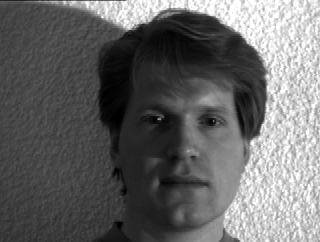
\includegraphics[scale=0.35]{Iluminacion1}
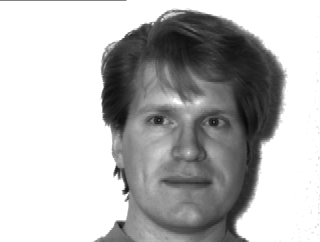
\includegraphics[scale=0.35]{Iluminacion2}
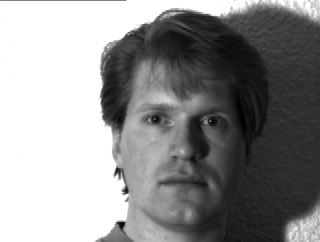
\includegraphics[scale=0.35]{Iluminacion3}
\caption{Ejemplos de la variación de la iluminación en un rostro. Extraídos de la base de datos "Yale A".}
\label{im:EjemIluminacion}
\end{figure}
\item \textit{Variación según el punto de visión}.- El rostro es un objeto tridimensional y debido al ángulo de visión de la cámara la apariencia del rostro puede variar debido a la deformación proyectiva, la cual lleva a que la parte inferior de rostro se vea más angosta de lo que realmente es (\cite{hill1997information}). Esto también se aplica para las rotaciones del rostro como se puede ver en la Figura \ref{im:EjemViewPoint}
\begin{figure}[h]
\center
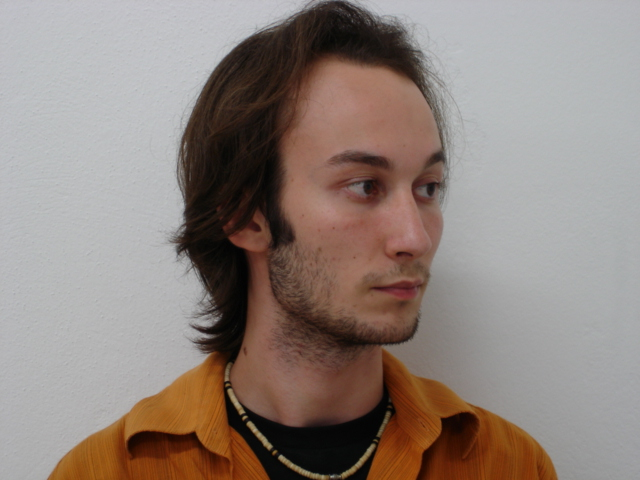
\includegraphics[scale=0.20]{ViewPoint1}
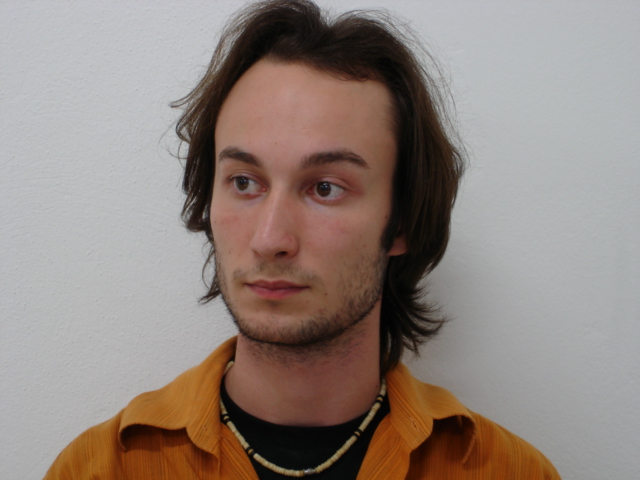
\includegraphics[scale=0.20]{ViewPoint2}
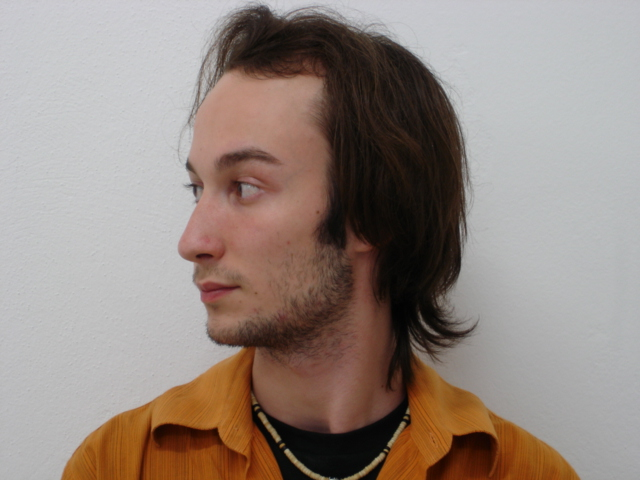
\includegraphics[scale=0.20]{ViewPoint3}
\caption{Ejemplos de como el punto de visión modifica un rostro. Extraídos de la base de datos "FEI".}
\label{im:EjemViewPoint}
\end{figure}
\item \textit{Expresión}.-  El rostro es un objeto no rígido, la expresión de la emociones es parte de la comunicación paralingüistica junto con el habla, y la variación de esas expresiones faciales influye en el reconocimiento del rostro. Ejemplos de ello se puede ver en la Figura \ref{im:EjemExpresion}
\begin{figure}[h]
\center
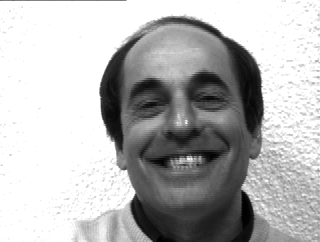
\includegraphics[scale=0.35]{Expresion1}
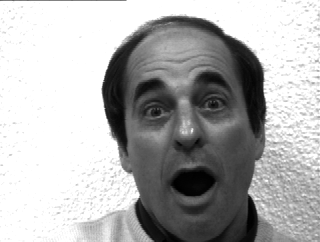
\includegraphics[scale=0.35]{Expresion2}
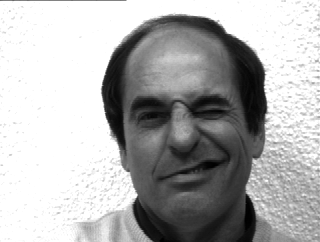
\includegraphics[scale=0.35]{Expresion3}
\caption{Ejemplos de la variación de la expresión en un rostro. Extraídos de la base de datos "Yale A".}
\label{im:EjemExpresion}
\end{figure}
\item \textit{Time delay}.- Es el intervalo de tiempo entre la adquisición de la imagen que se desea reconocer y la imagen o los datos con los cuales realizamos la identificación. Por ejemplo, intentar identificar a un sujeto el cual su ultima fotografía fue tomada hace un año.
\begin{figure}[h]
\center
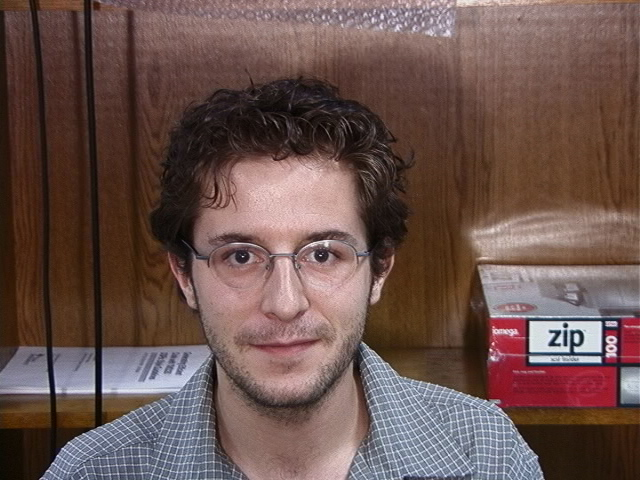
\includegraphics[scale=0.20]{Time1}
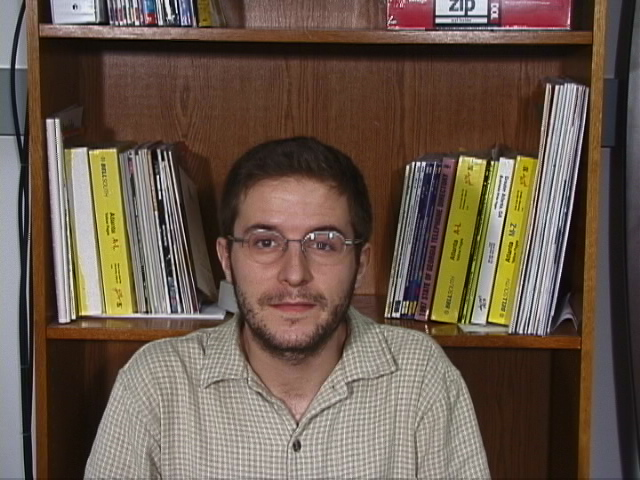
\includegraphics[scale=0.20]{Time2}
\caption{Ejemplos de la variación del tiempo en un mismo sujeto. Extraídos del la base de datos "Georgia".}
\label{im:EjemTimeDelay}
\end{figure}
\item \textit{Factores individuales}.- Se considera factores individuales a aquellos como el uso de maquillaje, estilos de peinado, disfraces, y otras formas en las que las personas modifican su apariencia a gusto personal. Un ejemplo de ello es el proyecto de ``CV Dazzle'' (\cite{harvey2014cv}) que usa el maquillaje para burlar las técnicas de detección de rostros como se puede ver en la Figura \ref{im:EjemMakeUp}.
\begin{figure}[h]
\center
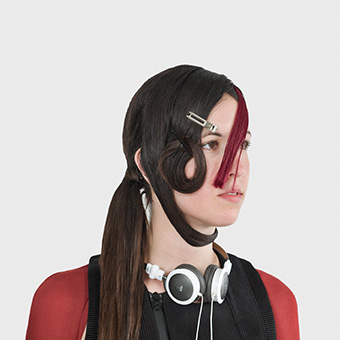
\includegraphics[scale=0.35]{MakeUp1}
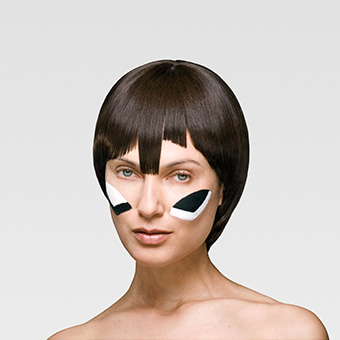
\includegraphics[scale=0.35]{MakeUp2}
\caption{Ejemplos extraídos del proyecto de ``CV Dazzle'' (\cite{harvey2014cv}).}
\label{im:EjemMakeUp}
\end{figure}
\item \textit{Oclusión}.- La oclusión puede darse debido a objetos en la escena o al uso de lentes de sol y otros objetos, también debido a la falta de cooperación de los individuos y a la variación según el punto de visión, Figura \ref{im:EjemOclusion}.
\begin{figure}[h]
\center
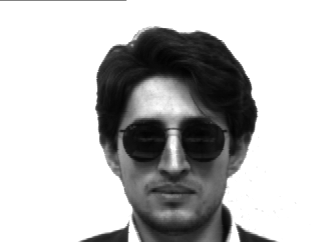
\includegraphics[scale=0.35]{Oclusion1}
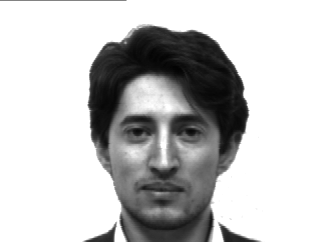
\includegraphics[scale=0.35]{Oclusion2}
\caption{Un ejemplo clásico de la oclusión del rostro es el uso de lentes de sol. Extraídos de la base de datos "Yale A".}
\label{im:EjemOclusion}
\end{figure}
\end{enumerate}

%Problemas de video vigilancia
A parte de los problemas listados, cuando el reconocimiento de rostros se aplica a  vídeo vigilancia surgen nuevas dificultades siendo las mas importantes:

\begin{enumerate}
\item \textit{La calidad del video}.- Debido a que la grabación de vídeo ocurre en ambientes no controlados todos los problemas anteriormente citados se presentan varias veces afectando la calidad final del vídeo. Cabe mencionar que a pesar de las mejora en resolución en las cámaras de vídeo vigilancia, frecuentemente se opta por equipos de gama baja en hogares y oficinas más como medida de disuasión que con el propósito de hacer vídeo vigilancia.
\item \textit{Falta de cooperación de los individuos}.- Es un problema que solo se presenta en vídeo vigilancia, debido a que en otros escenarios de reconocimiento de rostros como los presentados en la Tabla \ref{TaAplicaciones} siempre se puede esperar que las personas cooperen para ser identificas. Esto resulta ser uno de los motivos por el cual el reconocimiento de rostros es un problema de difícil resolución.
\item \textit{Las imágenes de los  rostros son pequeños}.- Debido a las condiciones de adquisición, las imágenes de los rostro son más pequeñas y de menor calidad de lo que asumen la mayoría de los sistemas de reconocimiento de rostros existentes. Por ejemplo, una región de rostros valida puede ser tan pequeña como 20$\times$20 pixeles, mientras los tamaños de las imágenes de los rostros usados en los sistemas actuales son tan grandes como 128$\times$128. El pequeño tamaño no solo hace la tarea de reconocimiento difícil, también afecta la precisión de la detección de puntos de interés que a menudo son necesarios en los métodos de reconocimiento.
\item \textit{Las características de los rostros como objetos}.- El rostro humano como objeto es más fácil de reconocer si se compara con otro objeto que no sea un rostro (diferencia Inter-clase) pero resulta mas difícil de reconocer si se le compara con otro rostro (diferencia Intra-clase) por ello detectar y localizar rostros es más fácil que reconocer un rostro en especifico (\cite{zhao2003face}). 
\end{enumerate}

%conclusion sobre seccion // mencionar biometria
Como se ha podido observar en esta sección el reconocimiento de rostros en vídeo vigilancia es una tarea muy difícil debido a la conjunción de varios factores, como el ambiente no controlado donde aparecen todas las dificultades relacionadas al típico reconocimiento de rostros. A ello se suma los problemas del escenario de video vigilancia en el cual se puede esperar la falta de cooperación de los sujetos a identificar y finalmente la calidad de los videos y las imágenes de los rostros.

Como parte de la propuesta expuesta en detalle en el Capítulo \ref{chap:Propuesta} intentamos resolver el problema de reconocimiento de rostros en un \textit{pipeline} de video vigilancia bajo las condiciones de una cámara de seguridad en alta definición, proponemos enfrentar las variaciones de iluminación a través de técnicas de pre-procesamiento, afrontar en parte el problema de variación de poses con el uso de los últimos avances en el \acf{CLNF} y \acf{EBGM} como método de reconocimiento biométrico. 

\section{Objetivos}\label{scc:Objetivos}

\subsection{Objetivo general}
Proponer un \textit{pipeline} para el reconocimiento de rostros en una escena de vídeo con la adaptación de \acf{CLNF} y \acf{EBGM} para su uso final en vídeo vigilancia.

\subsection{Objetivos específicos}
Como objetivos específicos se tiene:
\begin{itemize}
\item Comparar los diferentes métodos holísticos existentes contra \ac{EBGM}.
\item Analizar el impacto de la modificación de parámetros de \ac{EBGM}.
\item Analizar la influencia de incrementar el conjunto de entrenamiento mediante transformaciones de perspectiva en \ac{EBGM}.
\item Desarrollar los métodos de mejora del \textit{pipeline} propuesto con \ac{EBGM}.
\item Probar el \textit{pipeline} propuesto en imágenes de vídeo vigilancia.
%\item Verificar el efecto que tiene el uso de \ac{CLNF} como opción al método de localización de puntos fiduciales de \ac{EBGM}.
\end{itemize}

\section{Alcance y limites de la tesis}
A partir de los problemas mencionados en la Sección \ref{ssc:PlanteamientoProblema} la propuesta, explicada en el Capítulo \ref{chap:Propuesta} enfrenta los siguientes problemas:
\begin{itemize}
 \item Iluminación.- Con el uso del pre-procesamiento explicado en la Sección \ref{scc:PropIluminacion} que permite iluminar u oscurecer imágenes según  la situación lo requiera, de esta manera lograr una normalización el lo referente a iluminación cuando existe luz diurna.
 \item Variación según el punto de visión, Expresión facial.- Estos dos problemas son enfrentados con el uso de \ac{CLNF} como detector de puntos ya que como se muestra en el Capítulo \ref{chap:Resultados} mejora el rendimiento del reconocimiento. debido a su mayor exactitud en encontrar puntos fiduciales independientemente de las expresiones faciales.
\item Falta de cooperación de los individuos.- Es enfrentado mediante la unión del detector de Viola-Jones, detector de \ac{HOG}. También entra en consideración la posición de la cámara que fue puesta de formal tal que pueda captar los rostros de los transeúntes, Figura \ref{im:EscenaViola}.
\end{itemize}

Problemas como baja calidad del vídeo, imágenes de rostros muy pequeñas no son enfrentados con la propuesta, mas allá del pre-procesamiento y transformación de tamaña propio de \ac{EBGM} ya que no se emplea ninguna técnica de súper-resolutorio o mejora de imagen. Para el caso de oclusión y factores individuales no se propone ninguna mejora al funcionamiento de los detectores usados mas que su combinación para validar rostros y tampoco se prueba la propuesta cuando las imágenes de vídeo vigilancia  son de tomas de luz infrarroja.

\section{Organización de la tesis}
En los próximos capítulos se desarrollará el trabajo que comprende toda la tesis, en esta sección se realiza una breve descripción de cada uno de ellos.

\begin{enumerate}
\item En el Capítulo \ref{chap:Revision} se desarrolla una explicación del reconocimiento de rostros, una categorización de los métodos de reconocimiento de rostros, establecemos las diferencias entre métodos basados en características y métodos holísticos, donde se presenta el estado del arte en el reconocimiento de rostros.

\item En el Capítulo \ref{chap:Conceptos} se expone el marco teórico de nuestra propuesta. 
Se realiza una introducción a las técnicas de reconocimiento probadas en esta tesis, se profundiza el funcionamiento de \ac{EBGM} y se explica las razones de su uso para este trabajo. Definimos el concepto de biométria y cuales son los requerimientos para que un método de reconocimiento sea considerado biométrico.

\item En el Capítulo \ref{chap:Propuesta} se describe en detalle la propuesta de esta tesis, concentrándose en el \textit{pipeline} de vídeo desde la detección de rostros hasta el resultados del reconocimiento.

Se menciona el aporte de la modificación de \ac{EBGM} usando \ac{CLNF} para su adaptación al uso de vídeo vigilancia, junto al uso de mejoras en la iluminación.

\item En el Capítulo \ref{chap:Resultados} se muestran los resultados experimentales de la propuesta junto con las opciones exploradas para lograr el objetivo del trabajo de tesis.

\item Finalmente en el Capítulo \ref{chap:Conclusiones} se mencionan las conclusiones obtenidas en esta tesis y se listan los posibles trabajos futuros en continuación a este trabajo.
\end{enumerate}

Se ha expuesto el contexto y la necesidad de contar con propuestas par afrontar el trabajo de vídeo vigilancia en este trabajo, es necesario seguir resaltando su dificultad no solo para los algoritmos de visión computacional, sino para la personas en diversas situaciones.